
\vspace{10mm}

\part*{著者紹介}

\begin{wrapfigure}[5]{r}{3.5cm}
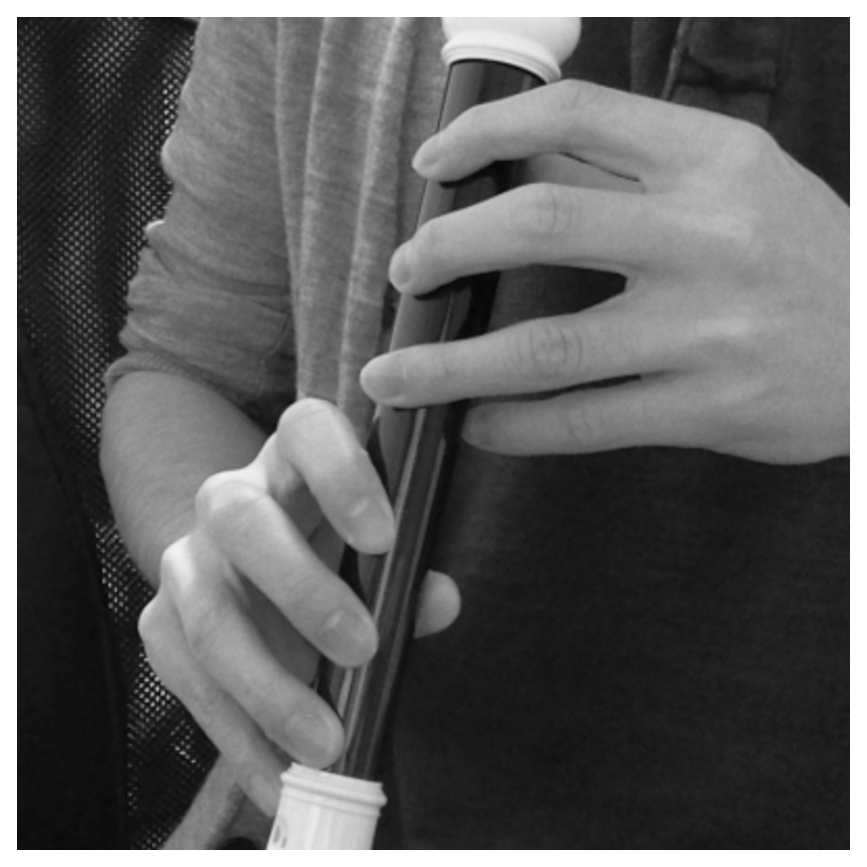
\includegraphics[width=3.5cm,clip]{res_author/tomoemon_temoto.eps}
\end{wrapfigure}
\section*{tomoemon}
twitter: \verb|@tomoemon|

本書の企画立ち上げと編集、各記事の推敲などをやらせていただきました。ここ最近はガチで練習していないのでタイパーを名乗るのはちょっと気が引けますが、心はいつでもタイパーです。特殊配列系タイパーとして(?)いろんな配列に手を出していましたが、tomoemon-AZIKという自己満足配列を生み出して一段落している今日この頃です。

\vspace{5mm}

\begin{wrapfigure}[5]{r}{3.5cm}
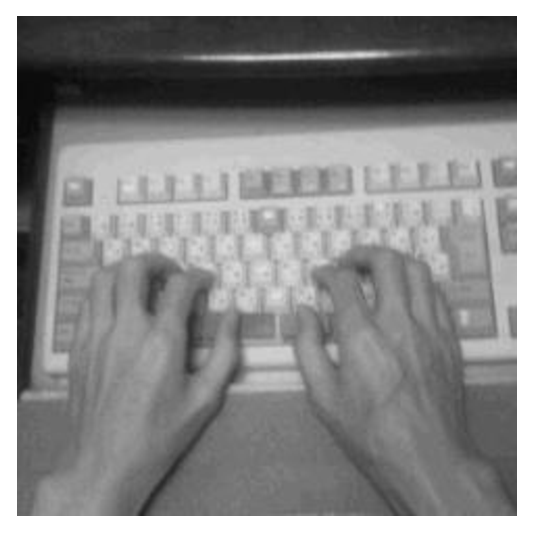
\includegraphics[width=3.5cm,clip]{res_author/kouy_temoto.eps}
\end{wrapfigure}
\section*{kouy}
twitter: \verb|@kouy|

配列作成者。2004年から新配列を使用し始め、親指シフト(NICOLA)、月配列2-263式、月配列U8版など巡り歩く。「月配列を文字キー同時打鍵で使いたい」という思いから配列作成の道に入り、下駄配列、けいならべ、新下駄配列を作成。ブログ『ローマ字入力でもなく、かな入力でもなく』http://kouy.exblog.jp/

\clearpage

\begin{wrapfigure}[7]{r}{3.5cm}
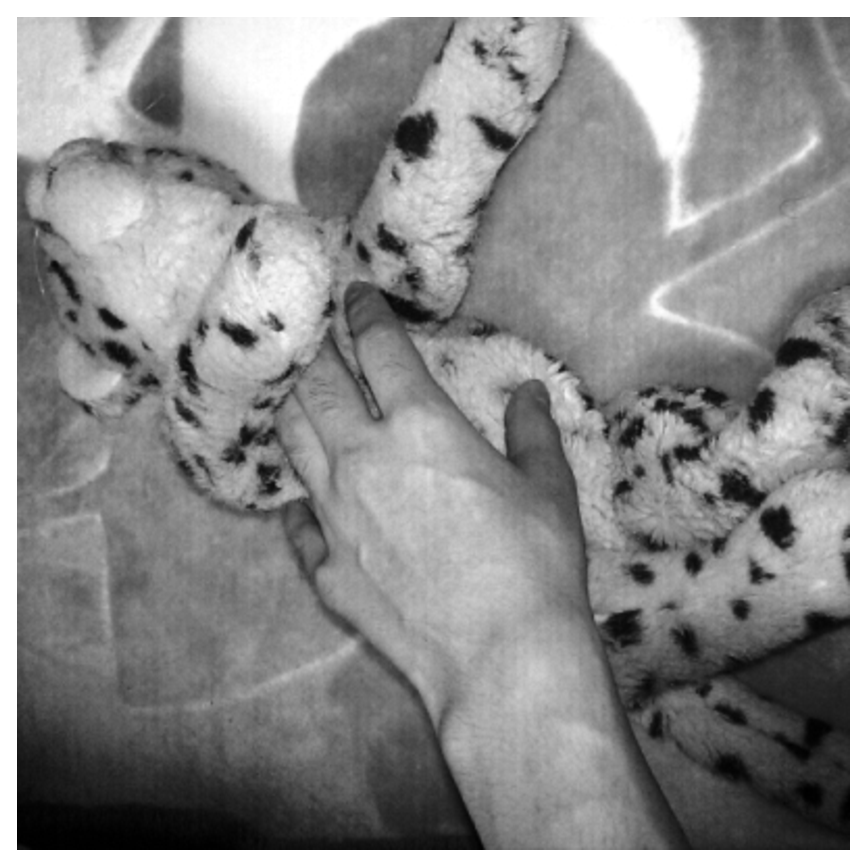
\includegraphics[width=3.5cm,clip]{res_author/vuttar_temoto.eps}
\end{wrapfigure}
\section*{テル}
twitter: \verb|@vuttar|

タイピングを始めて約13年。そのうち多くの時期をタイプウェルとともに過ごした、マゾヒスティックな練習オタク系タイパー。タイパーとしての特性は、理論派ではなく練習オタク・打ち分け以外の最適化無し・いわゆる標準運指・タイプウェル信者・オールラウンダー(JISかなや英語なども重視)・安定性重視など。使用キーボードはRealforce 91UBK 変荷重。保持記録は国語R総合ZF、国語K総合ZE、英単語総合ZEなど。

\vspace{5mm}

\begin{wrapfigure}[5]{r}{3.5cm}
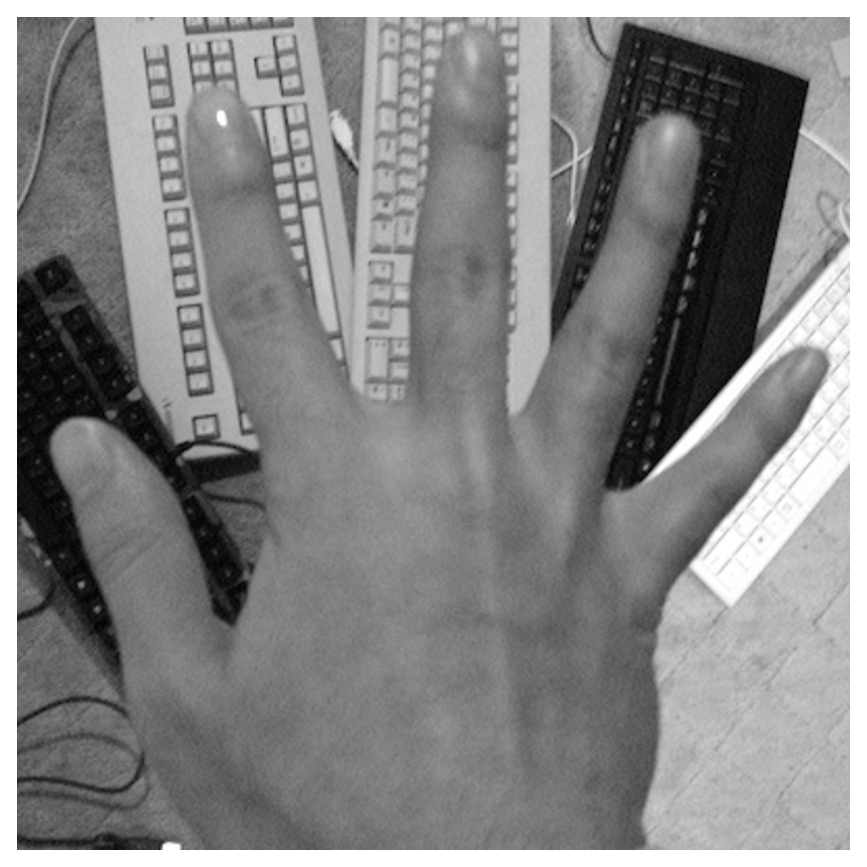
\includegraphics[width=3.5cm,clip]{res_author/eigh8_t_temoto.eps}
\end{wrapfigure}
\section*{eigh8\_t}
twitter: \verb|@eigh8_t|

配列からキーボード、コタツからバランスボールまで使えるものなら何でも使う環境系(?)タイパー。タイプウェルではお酒の力も借りながら国語RでZタイパーになりました。現在は配列系オールラウンダー目指し修行中。
 \\
 \\

\vspace{5mm}

\begin{wrapfigure}[6]{r}{3.5cm}
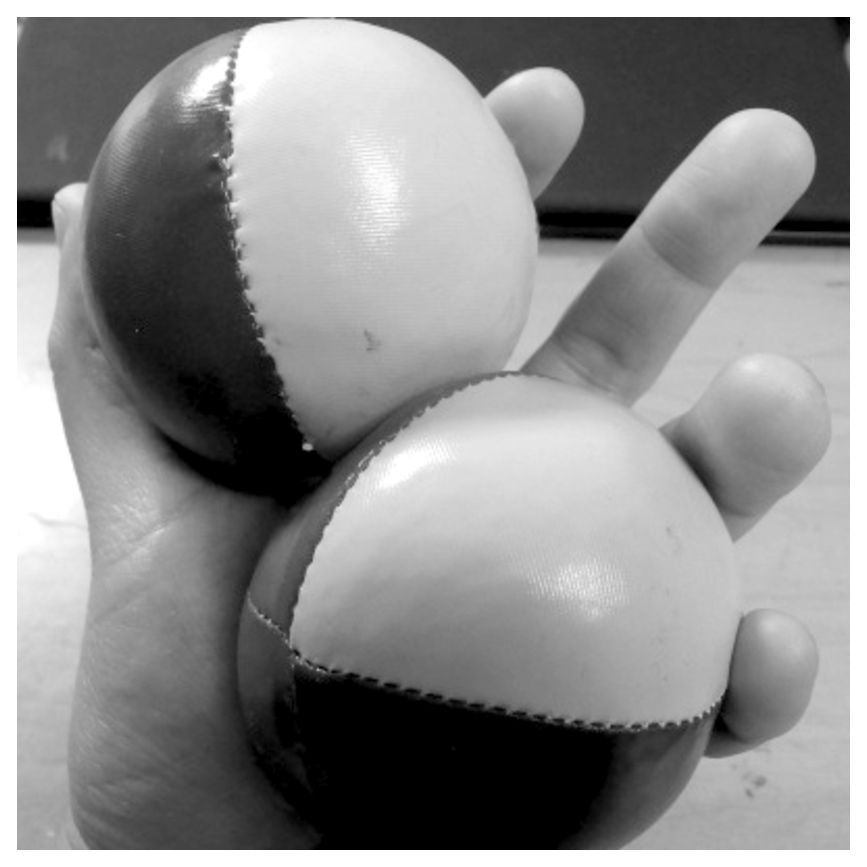
\includegraphics[width=3.5cm,clip]{res_author/nooyosh_temoto.eps}
\end{wrapfigure}
\section*{nooyosh}
twitter: \verb|@nooyosh|

言語と名のつくものが大好きな大学院生。大学では自然言語処理を専攻している。かじった言語はたくさんあるがどれも中途半端で身につかない。タイピングも好きだが、一方で文房具による手書きも大好きだったりする。現在はAZIK配列を改良してYAZIK: Yet another AZIKを作るのが目下の目標。

\vspace{5mm}

\begin{wrapfigure}[6]{r}{3.5cm}
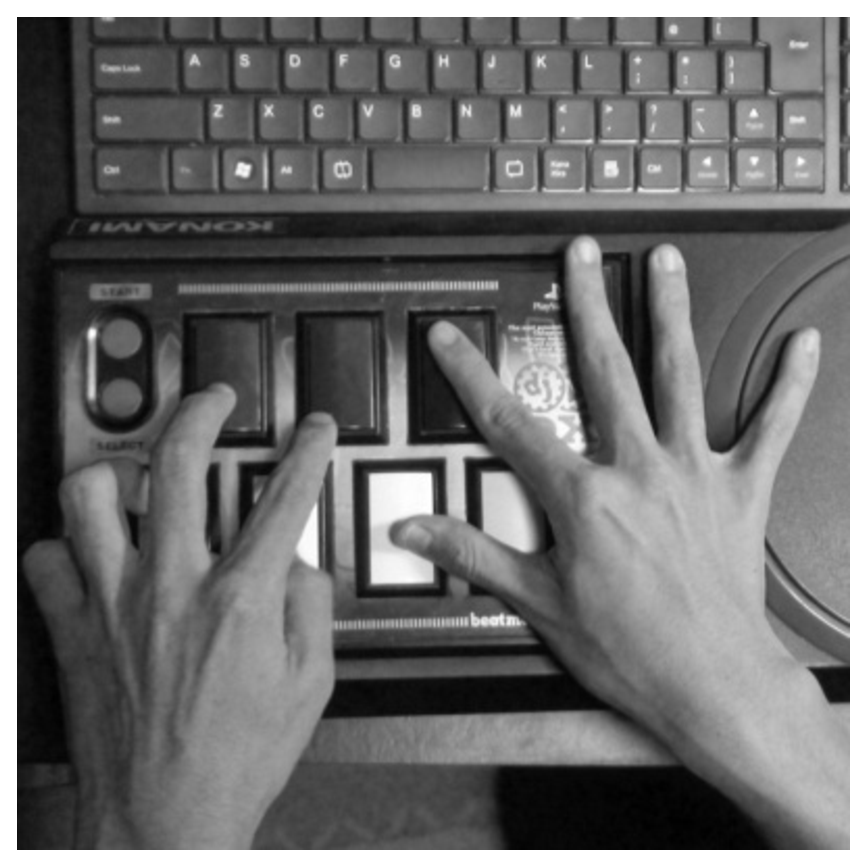
\includegraphics[width=3.5cm,clip]{res_author/ock_temoto.eps}
\end{wrapfigure}
\section*{o-ck}
twitter: \verb|@o_ck_SP_ANOTHER|

主に人差し指、中指を多用しまくる我流タイパー。'04年にタイプウェルと出会い、脇目も振らず我流運指の道を突き進んでいるうち、国語R総合1位を取っていたり('05年3月~'08年8月)。…というのも今は昔の話。そのうち音ゲーに走り始め、7つの鍵盤と1枚のお皿に全てを注ぎ込んでいた時期も。なにかと指先を使うスキルと縁があったのかもしれません。最近はDDRが楽しいです。

\vspace{5mm}

\begin{wrapfigure}[5]{r}{3.5cm}
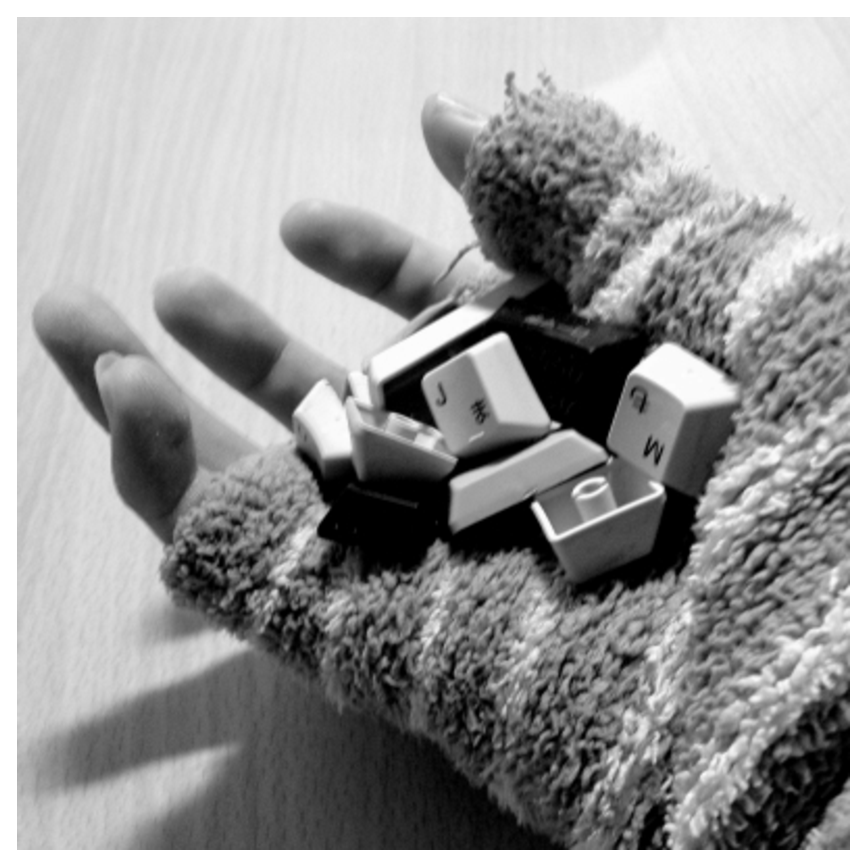
\includegraphics[width=3.5cm,clip]{res_author/x_i_temoto.eps}
\end{wrapfigure}
\section*{W/H}
twitter: \verb|@x_i|

有象無象の中の一名であったが、何やら書く中で色が染み、識別可能になったスライムベス的ギャラリータイパー。最近はすべキーを戯れに打つなど充実した余生を過ごしている。ゲーム開発・配列研究などにも幅広く手を出し、結果どれも中途半端になっているダメ勇者タイプ。他の趣味はノベルゲームや口笛。人生の目標は不老不死。20XX 年没。

